% 第12章第1节：构建问题与输出要求（作用域与依赖图、袋与接口、树分解与树宽、接口与内部变量、保留变量的结构要求）。

\section{构建问题与输出要求}
\label{sec:graph-dp-construction-problem}

第~\ref{sec:graph-dp-construction-goal}小节提出了一般图上动态规划的三项要求：每个局部项有处可放，接口足以概括内部变量，子问题的依赖可以排序。本节把这些要求写成可以核验的定义。先固定构建的输入，再引入袋与接口，用树分解刻画合法的袋树，并说明每个子问题的接口与内部变量；最后说明保留变量的查询对结构提出什么额外要求。

\subsection{作用域与依赖图}
\label{sec:graph-dp-scope-graph}

构建的输入只是变量集合$V$和各局部函数的作用域$S_a$，$a\in A$，不含任何函数值。由它们得到第~\ref{sec:graph-dp-factor-graphs}小节的原始图$\mathcal G=(V,E)$：以全部变量为顶点，两个变量同属某个作用域时连一条边。每个作用域$S_a$在$\mathcal G$中两两相邻。

顶点集取全部变量，包括不出现在任何局部函数中的孤立变量。这样的变量不带来成本，但最优配置仍要给它赋值，计数时也要累计它的全部状态，所以它仍须出现在结构中。四环算例的作用域就是四条边，原始图就是环$1-2-3-4-1$本身；三元作用域例子的原始图有五条边，只缺$\{1,4\}$。

构建只使用作用域，所得结构对作用域相同而数值任意的全部问题都适用。某组特定数值可能恰好使一张中间表还能进一步分解（第~\ref{sec:graph-dp-fill-in}小节给出一例），但构建不利用这种巧合：一般数值下必须保留的耦合，构建时一律保留。数值上的进一步化简要回到函数表本身判断，不属于本章的结构问题。

\subsection{袋与接口}
\label{sec:graph-dp-bags}

回到四环算例。第~\ref{sec:graph-dp-four-cycle}小节的计算先同时看$\{1,2,4\}$，产生以$\{2,4\}$为索引的表$\psi_1$；再同时看$\{2,3,4\}$，读入$\psi_1$完成计算。三元作用域例子也一样：若按次序$(1,4,2,3)$消元，消去$x_1$时要同时处理$\{1\}\cup S_1=\{1,2,3\}$，消去$x_4$时处理$\{2,3,4\}$，随后依次处理$\{2,3\}$和$\{3\}$。

每一步产生的新函数会在后面某一步被用到：$\psi_1$与$\psi_4$都在消去$x_2$时被合并，消去$x_2$得到的新函数在消去$x_3$时被使用。

把每一步同时处理的变量集合看成一个节点，按“新函数交给哪一步使用”连接这些节点，就得到图~\ref{fig:graph-dp-bags-interface}中间的一棵树。这棵树只记录了哪些变量要一起处理、表交给谁，与$\phi_A,\phi_B$的具体数值无关，换一组作用域相同的函数，它照样适用。

准备放进同一张表里同时索引的变量集合称为\term{袋}（bag），可以把它想成计算时一次摆上桌面的变量：对它们的每一种联合取值各记一个数。袋组成的树称为袋树。袋树的节点是计算单元，袋树的边表示两个计算单元之间传递一张表；它与原始图中连接两个变量的边含义不同。不同的袋可以有公共变量，例如$\{1,2,3\}$与$\{2,3,4\}$都含$2,3$。

\begin{figure}[!htb]
  \centering
  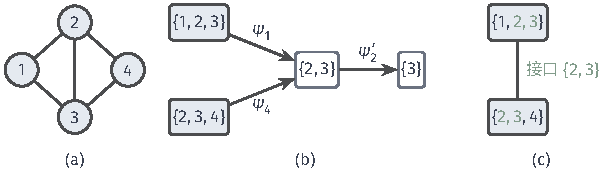
\includegraphics[width=103.283mm]{figures/01-basic-mathematics/04-graphs/tikz/c5-elimination-to-bags/figure.pdf}
  \caption{从消元步骤得到袋。左：三元作用域例子的原始图。中：按次序$(1,4,2,3)$消元时，每一步同时处理的变量集合构成一个袋，箭头表示新函数交给哪一步使用。右：$\{2,3\}$和$\{3\}$已包含在相邻的大袋中，并入后只剩两个袋，它们的交集$\{2,3\}$（绿色）就是接口。}
  \label{fig:graph-dp-bags-interface}
\end{figure}

袋与原始图中的团有关，但不必是团。原始图中两两相邻的顶点集合称为\term{团}（clique）。三元作用域例子中$\{1,2,3\}$是团，$\{1,2,4\}$不是，因为缺边$\{1,4\}$。四环算例中第一个袋$\{1,2,4\}$也不是原始图的团：$2$与$4$在环上不相邻，消去$x_1$后才通过$\psi_1$耦合。所以袋可以重叠，也可以含有原图中不相邻的变量。

\paragraph{接口与一致性}
在三元作用域例子中，袋$\{2,3\}$和$\{3\}$都已包含在相邻的大袋中，可以并入，最后只剩两个袋$\{1,2,3\}$与$\{2,3,4\}$，如图~\ref{fig:graph-dp-bags-interface}右侧。相邻两袋的交集称为它们的接口，这里是$\{2,3\}$；四环算例中两个袋的接口是$\{2,4\}$。这与第~\ref{sec:graph-dp-tree-idea}小节的接口变量含义相同，只是现在接口可以含多个变量。

接口上的变量在两个袋里是同一个变量，不是两个副本。左袋在汇总$x_1$时必须对$(x_2,x_3)$的每种取值分别给出结果，右袋使用这些结果时也必须按同样的$(x_2,x_3)$取值来读。左袋交出的正是一张以接口为索引的表。

两个袋之间只交换这样一张表，所以一个变量的取值也只能经接口从一个袋传到另一个袋，这就限制了袋的连接方式。若某个变量出现在两个不相邻的袋中，而连接它们的袋树路径上有某个袋不含这个变量，那么那个袋发出和收到的表都不以这个变量为索引，两侧便无法约定它取同一个值。另外，袋还必须能容纳所有局部函数，否则有的成本项无处计算。这两项要求合起来，就是下面的定义。

\subsection{树分解与树宽}
\label{sec:graph-tree-decomposition}
\label{sec:graph-dp-decomposition-definition}

在结构上，容纳局部函数的要求落实为每个变量和原始图的每条边都被某个袋包含；保持一致的要求就是上面的连接要求。

\begin{definition}[树分解]
\label{def:graph-dp-tree-decomposition}
设$\mathcal G=(V,E)$是有限无向图。$\mathcal G$的一个\term{树分解}（tree decomposition）由一棵有限树$\mathcal T$（节点集记为$T$）和每个节点$t\in T$上的子集$B_t\subseteq V$组成，满足：
\begin{enumerate}
  \item 顶点覆盖：每个顶点$v\in V$至少属于一个袋；
  \item 边覆盖：对每条边$\{u,v\}\in E$，存在某个袋同时含有$u$与$v$；
  \item 运行交集：对每个顶点$v\in V$，含$v$的节点集合$T_v=\{t\in T:v\in B_t\}$在$\mathcal T$中连通。
\end{enumerate}
第三个条件称为\term{运行交集性质}（running intersection property）。
\end{definition}

运行交集等价于：若$v$同时属于$B_s$和$B_t$，则$\mathcal T$中从$s$到$t$的路径上每个袋都含$v$。因为树中两点之间只有一条路径，$T_v$连通恰好意味着这条路径留在$T_v$中。直观地说，每个变量在袋树上占据一块连成一片的地盘；沿袋树行走，一个变量一旦离开就不会再出现。

\paragraph{梯子形图的分解}
图~\ref{fig:graph-dp-ladder-decomposition}中的梯子形图有两排顶点$1,2,3$与$4,5,6$，每排相邻顶点之间和同一列的两个顶点之间各有一条边。四个袋$\{1,2,4\},\allowbreak\{2,4,5\},\allowbreak\{2,3,5\},\allowbreak\{3,5,6\}$连成一条路径。

可以逐条核对定义。每个顶点都在某个袋中；七条边中，$\{1,2\},\{1,4\}$在第一个袋，$\{4,5\},\{2,5\}$在第二个袋，$\{2,3\}$在第三个袋，$\{5,6\},\{3,6\}$在第四个袋。

再看运行交集：含$2$的袋是前三个，含$5$的是后三个，含$4$的是前两个，含$3$的是后两个，都连成一段。

这个分解像一个窄窗口从左向右扫过梯子：每个袋是窗口某一时刻看到的顶点，相邻两袋的接口是窗口移动时必须记住的顶点。从第一个袋移到第二个袋时，$1$已经处理完毕，可以忘掉，只需记住$\{2,4\}$；之后$4$也处理完毕，只需记住$\{2,5\}$。运行交集保证被忘掉的顶点不会在后面的袋里再次出现，否则它的取值早已无从查找。梯子再长，窗口也只需同时看三个顶点；第~\ref{sec:graph-dp-chain}小节的链上递推是同样的扫描，只是每次只需记住一个变量。

\begin{figure}[!htb]
  \centering
  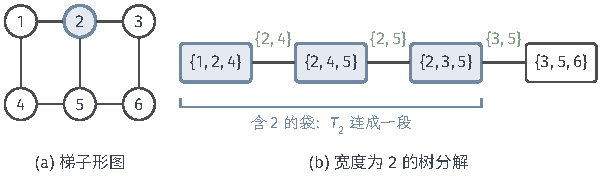
\includegraphics[width=101.85mm]{figures/01-basic-mathematics/04-graphs/tikz/c5-ladder-decomposition/figure.pdf}
  \caption{梯子形图的树分解。(a)两排顶点由三条横档相连。(b)四个袋连成一条路径，像窗口自左向右扫过梯子；边上的绿色集合是相邻两袋的接口，即窗口移动时要记住的顶点。蓝色的袋都含顶点$2$，它们连成一段，满足运行交集。}
  \label{fig:graph-dp-ladder-decomposition}
\end{figure}

\paragraph{运行交集的作用}
只覆盖顶点和边还不够。图~\ref{fig:graph-dp-running-intersection}比较路径$1-2-3-4$上的两种袋连接。两种连接使用同样的三个袋$\{1,2\},\allowbreak\{2,3\},\allowbreak\{3,4\}$，都覆盖了全部顶点和边。

上面一种按$\{1,2\}-\{2,3\}-\{3,4\}$连接，含$2$的两个袋相邻，含$3$的两个袋也相邻，是树分解。下面一种按$\{1,2\}-\{3,4\}-\{2,3\}$连接，含$2$的两个袋被不含$2$的袋$\{3,4\}$隔开。若沿这棵树计算，左端的袋可以选$x_2=0$，右端的袋可以选$x_2=1$，中间的袋不记录$x_2$，无从发现矛盾；拼起来的结果不对应任何一个配置。

\begin{figure}[!htb]
  \centering
  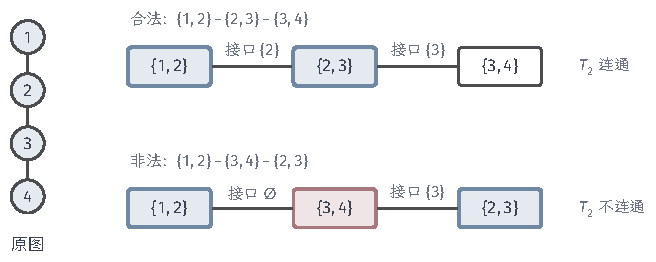
\includegraphics[width=111.016mm]{figures/01-basic-mathematics/04-graphs/tikz/c5-running-intersection/figure.pdf}
  \caption{路径$1-2-3-4$上的合法与非法袋连接。两种连接使用相同的三个袋，都覆盖全部顶点和边。上：含$2$的袋（蓝色）彼此相邻，含$3$的袋也相邻，满足运行交集。下：含$2$的两个袋之间隔着不含$2$的袋$\{3,4\}$（红色），$T_2$不连通，不是树分解。}
  \label{fig:graph-dp-running-intersection}
\end{figure}

\paragraph{宽度与树宽}
\label{sec:graph-dp-treewidth}
袋越大，袋表越大。为了用一个数概括一次分解的规模，定义树分解的宽度为
\[
\max_{t\in T}|B_t|-1,
\]
即最大袋的大小减一；图$\mathcal G$的\term{树宽}（treewidth）是它的全部树分解宽度的最小值，记为$\operatorname{tw}(\mathcal G)$。减一是一种约定，使得至少含一条边的树宽度恰为一。

把整个图放进一个袋总是合法的树分解，宽度为$|V|-1$，所以树宽总有定义，问题在于能否用更小的袋。直观地说，树宽回答的是：把这个图压成一棵树的形状时，每个树节点至少要装下多少个顶点。图越像树，需要的袋越小。

确定一个图的树宽需要两步：构造一个分解给出上界，再证明不存在更小宽度的分解给出下界。下面先给出几个小图的上界构造，图~\ref{fig:graph-dp-treewidth-examples}画出了相应的分解；下界的证明要用到第~\ref{sec:graph-dp-clique-containment}小节的团容纳引理，在那里补上。

单个顶点的图只需一个袋$\{1\}$，宽度为$0$，任何没有边的图都如此。至少含一条边的树有宽度为$1$的分解：任选根$\rho$，为每个非根顶点$u$建袋$\{u,p(u)\}$，其中$p(u)$是父点；若$p(u)$不是根，就把这个袋连到$p(u)$自己的袋上，根的各子点的袋则依次连成一条链。这样，非根顶点$v$出现在自己的袋和各子点的袋中，后者都与前者相邻；根只出现在各子点的袋中，它们连成链，所以运行交集成立。

四个顶点的环$1-2-3-4-1$有宽度为$2$的分解：两个袋$\{1,2,3\}$与$\{1,3,4\}$以一条边相连，接口为$\{1,3\}$；四环算例使用的$\{1,2,4\}$与$\{2,3,4\}$也是一个宽度为$2$的分解，接口为$\{2,4\}$。图~\ref{fig:graph-dp-ladder-decomposition}的梯子有宽度为$2$的分解。四个顶点两两相邻的完全图只用一个袋$\{1,2,3,4\}$，宽度为$3$。

\begin{figure}[!htb]
  \centering
  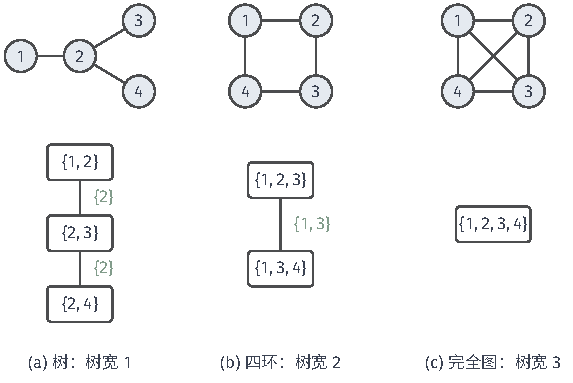
\includegraphics[width=96.95mm]{figures/01-basic-mathematics/04-graphs/tikz/c5-treewidth-examples/figure.pdf}
  \caption{三个四顶点图及其宽度最小的树分解，绿色集合是接口。(a)树：每条边一个袋，宽度为$1$。(b)四环：任何分解都有一个袋含三个顶点，宽度为$2$。(c)完全图：全部顶点必须同在一个袋中，宽度为$3$。}
  \label{fig:graph-dp-treewidth-examples}
\end{figure}

某一次构造得到宽度$k$，只说明$\operatorname{tw}(\mathcal G)\leq k$；要断言树宽恰为$k$，还需要证明不存在更小宽度的分解。

若每个变量至多有$q$个状态，宽度为$k$的分解中，每个袋至多有$k+1$个变量，稠密存储的袋表至多$q^{k+1}$项。这是第~\ref{chap:general-graph-dp-computation}章中主要的枚举规模。实际的总开销还包括袋的个数、接口的大小和每次读取局部函数的成本，宽度只控制其中随状态数指数增长的那一部分，第~\ref{sec:graph-dp-computation-cost}节再作完整分析。

寻找树宽最小的分解与使用一个已经给定的分解是两项不同的任务。前者在一般图上是困难的组合问题；后者只需按定义核验三个条件，再沿树计算。第~\ref{sec:graph-tree-decomposition-construction}节给出的构造方法都只保证得到合法的分解和宽度上界。

\subsection{接口与内部变量}
\label{sec:graph-dp-interface-internal}

一个树分解还要选定根，才能确定子问题的依赖次序。设已给袋树选根$r$，每个非根节点$u$有父节点$p(u)$。称
\[
S_u=B_u\cap B_{p(u)}
\]
为$u$的接口，$I_u=B_u\setminus S_u$为$u$的\term{内部变量}（internal variable）。根没有父节点，约定$S_r=\varnothing$、$I_r=B_r$。

节点$u$对应的子问题是：固定接口取值$\bm x_{S_u}$，汇总内部变量$\bm x_{I_u}$以及$u$下方各子问题已经汇总的内容，输出一张以$\bm x_{S_u}$为索引的表，交给父节点。接口为空时，这张表只有一项，是一个数。四环算例以$\{2,3,4\}$为根时，子节点$\{1,2,4\}$的接口为$\{2,4\}$，内部变量为$\{1\}$；根的内部变量为$\{2,3,4\}$。

为了让每个变量恰好被汇总一次，每个变量应当恰好是一个节点的内部变量。下面的引理说明运行交集保证了这一点，并指出是哪个节点。

\begin{lemma}[每个变量恰在一个袋中作内部变量]
\label{lem:graph-dp-unique-internal}
设$(\mathcal T,\{B_t\}_{t\in T})$是$\mathcal G$的树分解，袋树以$r$为根。对每个$v\in V$，$T_v$中有唯一一个离根最近的节点，记为$\operatorname{top}(v)$，$T_v$的每个节点都是它的后代（含它本身）；并且$v\in I_u$当且仅当$u=\operatorname{top}(v)$。
\end{lemma}

\begin{proof}
由顶点覆盖，$T_v$非空。取$T_v$中深度最小的一个节点$t$。若$y\in T_v$不是$t$的后代，从$y$到$t$的树上路径要先向上经过$y$与$t$的最近公共祖先$z$，而$z$比$t$更靠近根；由$T_v$连通，这条路径留在$T_v$中，于是$z\in T_v$，与$t$的选取矛盾。所以$T_v$的节点都是$t$的后代，深度最小的节点也只有$t$一个，记$\operatorname{top}(v)=t$。

若$u=\operatorname{top}(v)$是根，则$v\in B_r=I_r$。若它不是根，其父节点不是它的后代，因而不在$T_v$中，即$v\notin B_{p(u)}$，所以$v\in I_u$。反过来，若$u\in T_v$而$u\neq\operatorname{top}(v)$，则$u$是$\operatorname{top}(v)$的真后代，从$u$到$\operatorname{top}(v)$的路径第一步就到达$p(u)$；由运行交集，$p(u)\in T_v$，所以$v\in S_u$，不是$u$的内部变量。
\end{proof}

由此，构建的结果应当记录每个节点的袋$B_u$、父节点$p(u)$、接口$S_u$和内部变量$I_u$。这些都是结构信息；节点上要汇总哪些局部函数、汇总出的表取什么值，在第~\ref{chap:general-graph-dp-computation}章求值时确定。

\subsection{保留变量的结构要求}
\label{sec:graph-dp-query-structure}

第~\ref{sec:graph-dp-problem}小节的另一种输出是保留集$R\subseteq V$上的条件最小成本表$F_R(\bm x_R)$。这张表以$\bm x_R$的联合取值为索引，所以必须有某个计算单元同时看到$R$中的全部变量，并且在那之前不能把$R$中的任何变量汇总掉。

结构上采用两条要求。第一，在原始图中把$R$补成团，即在$R$的任意两个不相邻的变量之间加边，得到图$\mathcal G_R$，再为$\mathcal G_R$构建结构。第二，选取的根袋包含$R$。由第~\ref{sec:graph-dp-clique-containment}小节的团容纳引理，$\mathcal G_R$的任一树分解都有某个袋包含$R$，可以选它作根。

根袋包含$R$以后，$R$中每个变量$v$的$\operatorname{top}(v)$都是根，由引理~\ref{lem:graph-dp-unique-internal}，它们不会成为任何非根节点的内部变量，因而不会提前被汇总。根处只汇总$B_r\setminus R$，留下以$\bm x_R$为索引的表。用变量消元描述时，这相当于只消去$V\setminus R$中的变量，最后保留$R$（第~\ref{sec:graph-dp-order-to-decomposition}小节）。

补边可能增大宽度。路径$1-2-3$的树宽为$1$，若$R=\{1,3\}$，补边后得到三角形，树宽变为$2$。所以带保留变量的任务，其宽度要按$\mathcal G_R$计算，不能直接沿用不带查询时的最小树宽；输出表本身还有$\prod_{i\in R}|\mathcal X_i|$项。

在四环算例中取$R=\{1,3\}$。$1$与$3$在环上不相邻，补边$\{1,3\}$后，$\{1,2,3\},\{1,3,4\}$构成宽度为$2$的分解，两个袋都含$R$，任选一个作根即可。原来使用的分解$\{1,2,4\}-\{2,3,4\}$则没有袋同时含$1$和$3$，不能直接回答这个查询。

两个边界情形是：$R=\varnothing$时不加任何要求；$R=V$时$\mathcal G_R$是完全图，任何分解都有一个袋含全部变量，宽度为$n-1$，这与输出表本身就要列出全部配置一致。
